Que haya un árbol $G$ de $n$ vértices, con una raíz arbitraria. La esencia de esta descomposición del 
árbol es dividir el árbol en varios caminos para que podamos llegar al vértice de la raíz desde cualquier
$v$ atravesando como máximo $\log n$ caminos. Además, ninguno de estos caminos debe cruzarse con otro.

Está claro que si encontramos tal descomposición para cualquier árbol, nos permitirá reducir ciertas 
consultas individuales de la forma \emph{calcular algo en el camino desde $a$ a $b$} a varias consultas 
del tipo \emph{calcular algo en el segmento $[l,r]$ del $k^{th}$ camino}.

Calculamos para cada vértice $v$ el tamaño de su subárbol $s(v)$, es decir, el número de vértices en el 
subárbol del vértice $v$ incluyéndose a sí mismo.

A continuación, considere todas las aristas que conducen a los hijos de un vértice $v$ Llamamos pesada a 
una arista si conduce a un vértice $c$ tal que:

$$s(c) \ge \frac{s(v)}{2} \iff \text{arista}(v,c)\text{ es pesada}$$

Todos los demás aristas están etiquetados como ligeras.

Es obvio que a lo sumo una arista pesada puede emanar de un vértice hacia abajo, porque de lo contrario 
el vértice $v$ tendría al menos dos hijos de tamaño $\ge\frac{s(v)}{2}$ , y por lo tanto el tamaño del 
subárbol de $v$ sería demasiado grande, $s(v) \ge 1 + 2 \frac{s(v)}{2} > s(v)$, lo que conduce a una 
contradicción.

Ahora descompondremos el árbol en caminos disjuntos. Considere todos los vértices de los que no 
descienden aristas pesadas. Subiremos desde cada uno de esos vértices hasta llegar a la raíz del árbol 
o pasar por una arista ligera. Como resultado, obtendremos varias rutas que se componen de cero o más 
aristas pesadas más una arista ligera. El camino que termina en la raíz es una excepción a esto y no 
tendrá una arista ligera. Dejemos que estos se llamen caminos pesados : estos son los caminos deseados 
de descomposición pesado-ligero.

Primero, notamos que los caminos pesados obtenidos por el algoritmo serán \textbf{disjuntos}. De hecho, si dos de estos caminos tienen una arista común, implicaría que hay dos aristas pesadas saliendo de un 
vértice, lo cual es imposible.

En segundo lugar, mostraremos que bajando desde la raíz del árbol hasta un vértice arbitrario, cambiaremos no más de $\log n$ caminos pesados a lo largo del camino. Bajar por una arista ligera reduce el tamaño del subárbol actual a la mitad o menos:

$$s(c) < \frac{s(v)}{2} \iff \text{arista}(v,c)\text{ es ligera}$$

Así, podemos pasar como máximo $\log n$ aristas ligeras antes de que el tamaño del subárbol se reduzca a uno.

Dado que podemos movernos de un camino pesado a otro solo a través de una arista ligera (cada camino pesado, excepto el que comienza en la raíz, tiene una arista ligera), no podemos cambiar los caminos pesados más de$\log n$ veces a lo largo del camino desde la raíz hasta cualquier vértice, según se requiera.

La siguiente imagen ilustra la descomposición de un árbol de muestra. Los bordes gruesos son más gruesos que las aristas ligeras. Los caminos pesados están marcados por límites punteados.

% TODO: \usepackage{graphicx} required
\begin{figure}[h!]
	\centering
	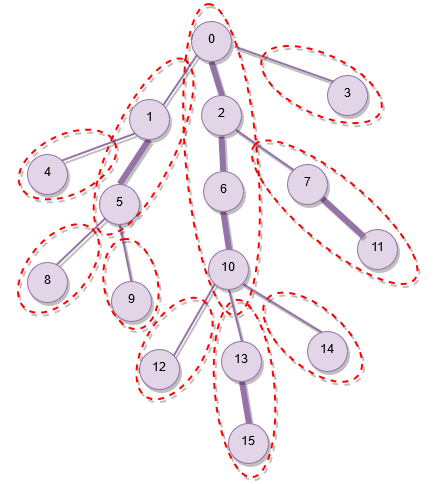
\includegraphics[width=0.5\linewidth]{img/hld}
	%\caption{}
	\label{fig:hld}
\end{figure}

Ciertas partes del enfoque discutido anteriormente pueden modificarse para facilitar la implementación sin perder eficiencia.

\begin{itemize}
	\item La definición de \textbf{arista pesada} se puede cambiar al arista que lleva al hijo con el subárbol más grande, con los lazos rotos arbitrariamente. Esto puede resultar en que algunas aristas ligeras se conviertan en pesadas, lo que significa que algunas rutas pesadas se combinarán para formar una sola ruta, pero todas las rutas pesadas permanecerán separadas. También se garantiza que descender por una arista ligera reduce el tamaño del subárbol a la mitad o menos.
	\item En lugar de construir un árbol de rangos sobre cada ruta pesada, se puede usar un árbol de un solo rango con rangos separados asignados a cada ruta pesada.
	\item Se ha mencionado que responder consultas requiere el cálculo del LCA. Si bien LCA se puede calcular por separado, también es posible integrar el cálculo de LCA en el proceso de respuesta a consultas.
\end{itemize}